% Implementacioni model i struktura

Иако нам математички модели дају прецизну дефиницију динамичких графова, они нису увек погодни за практичну примену због своје сложености. Наиме, често се у пракси очекује да знамо тренутно стање графа, без потребе за корацима који су до тог стања довели. Поред тренутног стања пожељно је и да се одржавају одређена својства графа, зависно од потреба проблема. У овом поглављу биће представљен једноставнији модел динамичких графова који је погодан за имплементацију, као и структура података која се користи у имплементацији.

\section{Ограничења формалног модела и поједностављен модел}

Директна примена прецизног математичког модела у практичним системима има значајна ограничења. Пре свега, овај модел подразумева чување комплетног стања графа за сваки временски тренутак, што доводи до велике просторне сложености, која је реда $O(|T| \cdot (|V| + |E|))$. Поред тога, у одсуству експлицитних информација о ажурирањима, прелаз између узастопних стања захтева поређење комплетних структура или поновно израчунавање својстава графа, што је рачунски неефикасно.

Даље, овакав модел није у складу са начином на који се промене јављају у реалним системима, где се оне појављују као појединачна ажурирања, а не као комплетне верзије графа. Због тога модели који не подржавају ефикасну обраду ажурирања и инкрементално одржавање својстава графа имају ограничену практичну примену \cite{islam2024dgapefficientdynamicgraph}.

Из свих наведених разлога, у практичним применама се користе поједностављени модели који се фокусирају на одржавање тренутног стања графа и подршку ефикасним ажурирањима.

У наставку се разматра један такав модел, у којем се динамички граф посматра искључиво кроз своје тренутно стање, без експлицитног чувања историје промена. За његову имплементацију користи се структура података \emph{хеш-индексираних блокова суседства} (енгл. \textit{Dynamic Hashed Blocks - DHB}) \cite{vandergrinten_et_al:LIPIcs.SEA.2022.11}. Пре него што детаљно обрадимо DHB структуру, биће представљено неколико других поједностављених модела који се користе у литератури, као и разлози за избор DHB структуре у овој имплементацији.

\section{Постојећи поједностављени модели}


Стандардни модели за представљање графова укључују листе суседства и матрице суседства. Међутим, ови модели нису погодни за динамичке графове због неефикасних ажурирања структуре.

У контексту динамичких графова, разматрају се два основна циља. Први циљ је постизање високе брзине ажурирања уз минималну потрошњу меморије. Други циљ је убрзавање алгоритама који се извршавају над графом ради анализе његове структуре и својстава. Већина постојећих приступа фокусира се превасходно на први циљ, занемарујући ефикасност алгоритама \cite{vandergrinten_et_al:LIPIcs.SEA.2022.11}.

Ради превазилажења ових ограничења, у литератури су анализиране различите структуре података које се могу користити за представљање динамичких графова. Иако је број ових структура велики и свака има своје специфичне предности и недостатке, неке од најпознатијих су:

\begin{itemize}
    \item \textit{Компресовани ретки редови} (енгл. \textit{Compressed Sparse Row - CSR}) - компактна репрезентација са просторном сложеношћу $O(|V| + |E|)$. Погодна за статичке графове, али непогодна за честа ажурирања \cite{wheatman2018packed,islam2024dgapefficientdynamicgraph}.
    \item \textit{STINGER} (\textit{Spatio-Temporal Interaction Networks and Graphs Extensible\\ Representation}) - динамичка структура заснована на блоковима повезаним у листе, са подршком за паралелно извршавање. Омогућава ефикасна ажурирања и анализу великих графова, али је сложенија за имплементацију \cite{ediger2012stinger}.
    \item \textit{Хеш индексирани блокови суседства} - блоковска структура са хеш индексом који омогућава брз приступ суседима. Представља компромис између ефикасности ажурирања и сложености имплементације \cite{vandergrinten_et_al:LIPIcs.SEA.2022.11}.
\end{itemize}

Иако свака од наведених структура има своје предности, CSR није погодан за динамичке графове због скупих ажурирања, док STINGER, иако веома ефикасан, уводи значајну имплементациону сложеност. Структура \emph{хеш-индексираних блокова суседства} представља компромис између ова два приступа, задржавајући добре перформансе уз знатно једноставнију имплементацију, због чега је изабрана за даљу анализу и реализацију.

\section{DHB структура}

Структура података \emph{хеш-индексираних блокова суседства} (DHB) је заснована на блоковима меморије са додатним хеш индексом за убрзање приступа суседима и проверу постојања грана. Иако се ослања на једноставне механизме управљања меморијом, експериментални резултати приказани у раду \cite{vandergrinten_et_al:LIPIcs.SEA.2022.11} показују да DHB постиже перформансе које су упоредиве са савременим динамичким и статичким оквирима, а у многим сценаријима их и превазилази. Конкретно, у једнонитном режиму рада DHB остварује у просеку 1,9 до 9,4 пута већу брзину уметања грана у поређењу са водећим савременим решењима заснованим на стаблима и хибридним структурама, као и статичким низовима суседства, док је од системa заснованих на блоковима бржи и до неколико десетина пута.

DHB је дизајниран тако да су операције које су од значаја за рад са динамичким графовима ефикасне. Ове операције укључују \cite{vandergrinten_et_al:LIPIcs.SEA.2022.11}:
\begin{itemize}
    \item Основне операције - DHB даје стандардни интерфејс за рад са графовима који подржава следеће операције: додавање и уклањање чворова и грана, промену тежина грана, проверу постојања грана и итерацију кроз суседе. 
    \item Произвољан распоред суседа - одређени алгоритми захтевају да суседи буду распоређени на одређени начин како би радили исправно (нпр. алгоритам Suitor\footnote{Suitor је похлепни алгоритам за апроксимацију максималног упаривања који током извршавања користи уређен обилазак суседа. Биће детаљније описан у поглављу \ref{chp:algoritmi}.}). Како би ово било омогућено, структура података не би требало да намеће фиксни распоред суседа. DHB захваљујући свом дизајну омогућава произвољно преуређивање суседа, што га чини погодним за алгоритме који захтевају специфичан редослед суседа.
    \item Подршка за конкурентно извршавање - многи алгоритми за рад са динамичким графовима подразумевају паралелну обраду суседа различитих чворова. DHB ово омогућава коришћењем појединачних хеш индекса за сваки чвор чиме се омогућава конкурентно извршавање. 
    \item Насумичан приступ - многи алгоритми очекују да могу приступити $i$-том ($i \in [0, \deg(u))$) суседу чвора $u$ у константном времену, на пример када се приступа насумичном суседу. DHB подржава овај захтев тако што суседе чува секвенцијално у низу, што омогућава директан индексни приступ. 
\end{itemize}

DHB је дизајниран тако да сваки чвор у графу садржи блок у коме су уписани његови суседи. Сваки блок садржи низ суседа као и хеш индекс који омогућава брзу проверу постојања и позицију суседа. Овај дизајн омогућава једноставно управљање и ажурирање суседства, као и ефикасно итерирање кроз суседе. Прецизније, сваки чвор садржи следећа поља \cite{vandergrinten_et_al:LIPIcs.SEA.2022.11}:

\begin{itemize}
    \item $deg(u)$ - тренутни степен чвора $u$, односно број његових суседа.
    \item $\beta$(u) - позитиван цео број који представља тренутну величину блока суседа чвора $u$.
    \item Низ суседа $N(u)$ - низ који садржи суседе чвора $u$, где првих $\deg(u)$ позиција садржи тренутне суседе, а остатак је празан.
    \item Хеш индекс $H(u)$ - структура која омогућава брзу проверу постојања суседа чвора $u$.
\end{itemize}

Како би се олакшало одржавање хеш индекса, величина блока суседа $\beta$(u) је увек степен двојке. Ово омогућава ефикасно управљање блоковима и брзо израчунавање позиције суседа у низу. Такође, увек је гарантовано да је $deg(u) \leq \beta(u)$. Због тога је у низу суседа првих $deg(u)$ позиција увек заузето, док су преостале позиције празне и спремне за нове суседе који ће бити додати у будућности \cite{vandergrinten_et_al:LIPIcs.SEA.2022.11}.

Коначно, граф је представљен као низ хеш-индексираних блокова суседства, где је сваки блок везан за одређени чвор. На слици \ref{fig:dhb_structure} је приказана структура података DHB. 

\begin{figure}[h]
\centering
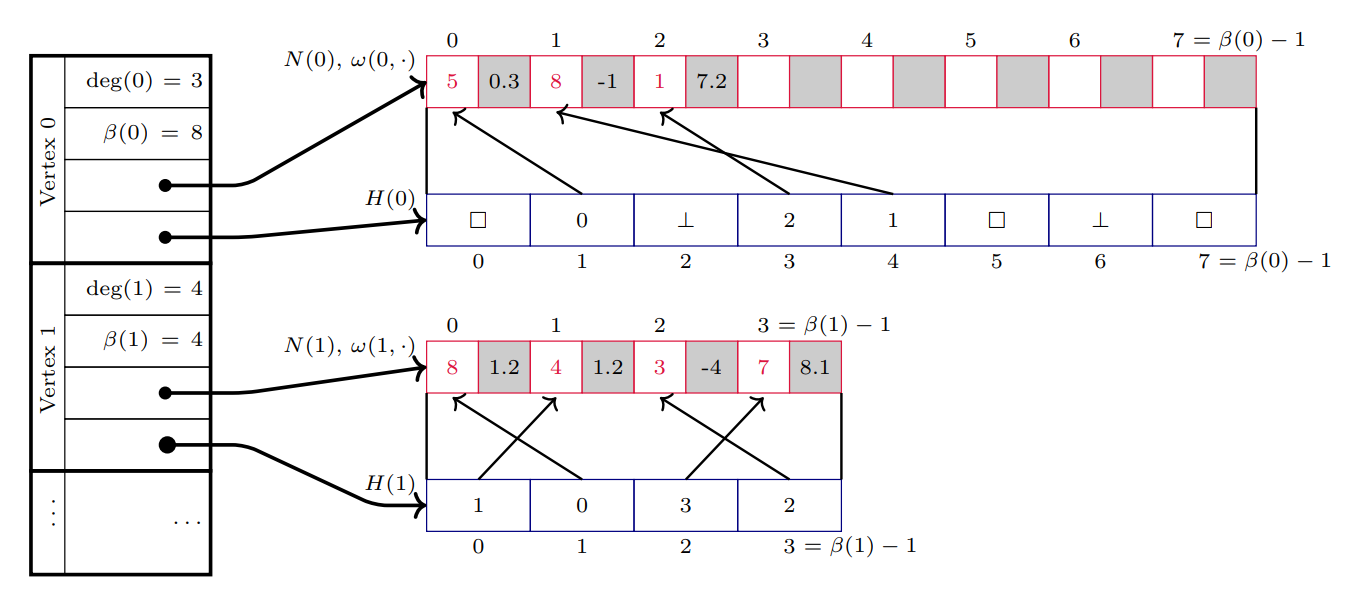
\includegraphics[width=1\textwidth]{images/layout_of_dhb.png}
\caption{Структура хеш-индексираних блокова суседства (DHB) \cite{vandergrinten_et_al:LIPIcs.SEA.2022.11}}
\label{fig:dhb_structure}
\end{figure}


\begin{example}
    Граф са слике \ref{fig:primer_dinamickog_grafa1} можемо једноставно представити DHB структуром. Како граф има четири чвора, потребна су нам четири блока суседства. Додавањем грана у граф ови блокови мењају своје величинe и садржај. На слици \ref{fig:dhb_jedna_grana} приказана је DHB структура након додавања гране $(1, 2)$, док на слици \ref{fig:dhb_sve_grane} видимо стање структуре након додвања свих преосталих грана. Приметимо да се величина блока првог чвора повећала са 2 на 4 након додавања гране $(1, 3)$, док су величине блокова осталих чворова остале непромењене.
\end{example}

\begin{figure}[htbp]
\centering
\begin{tikzpicture}[
    scale=0.85, every node/.style={transform shape},
    box/.style={draw, minimum height=0.6cm, minimum width=0.6cm, inner sep=0pt, align=center, font=\small},
    emptybox/.style={draw, fill=gray!10, minimum height=0.6cm, minimum width=0.6cm, inner sep=0pt, align=center, font=\small},
    headbox/.style={draw, minimum height=0.6cm, minimum width=1.8cm, inner sep=2pt, align=center, font=\footnotesize},
    titlebox/.style={draw, fill=gray!20, minimum height=1.2cm, minimum width=0.8cm, align=center, font=\bfseries\small},
    arrow/.style={->, >=stealth, thick}
]

% ==================== ЧВОР 1 ====================
\node[titlebox] (v1) {Vertex\\1};
\node[headbox, right=0cm of v1.north east, anchor=north west] (v1_deg) {$\deg(1) = 1$};
\node[headbox, right=0cm of v1.south east, anchor=south west] (v1_beta) {$\beta(1) = 2$};

% N(1) array
\node[box, right=1.5cm of v1_deg.east, anchor=west] (n1_0) {\textcolor{red!70!black}{2}};
\node[emptybox, right=0cm of n1_0] (n1_1) {};

\node[above=0.05cm of n1_0, font=\tiny] {0};
\node[above=0.05cm of n1_1, font=\tiny] {1};
\node[left=0.1cm of n1_0, font=\small] {$N(1)$};

% H(1) table
\node[box, below=0.6cm of n1_0] (h1_0) {0};
\node[emptybox, right=0cm of h1_0] (h1_1) {$\square$};

\node[below=0.05cm of h1_0, font=\tiny] {0};
\node[below=0.05cm of h1_1, font=\tiny] {1};
\node[left=0.1cm of h1_0, font=\small] {$H(1)$};

\draw[arrow] (v1_beta.east) -- (n1_0.west);
\draw[arrow] (h1_0.north) -- (n1_0.south);


% ==================== ЧВОР 2 ====================
\node[titlebox, below=1.6cm of v1.south west, anchor=north west] (v2) {Vertex\\2};
\node[headbox, right=0cm of v2.north east, anchor=north west] (v2_deg) {$\deg(2) = 0$};
\node[headbox, right=0cm of v2.south east, anchor=south west] (v2_beta) {$\beta(2) = 2$};

% N(2) array
\node[emptybox, right=1.5cm of v2_deg.east, anchor=west] (n2_0) {};
\node[emptybox, right=0cm of n2_0] (n2_1) {};

\node[above=0.05cm of n2_0, font=\tiny] {0};
\node[above=0.05cm of n2_1, font=\tiny] {1};
\node[left=0.1cm of n2_0, font=\small] {$N(2)$};

% H(2) table
\node[emptybox, below=0.6cm of n2_0] (h2_0) {$\square$};
\node[emptybox, right=0cm of h2_0] (h2_1) {$\square$};

\node[below=0.05cm of h2_0, font=\tiny] {0};
\node[below=0.05cm of h2_1, font=\tiny] {1};
\node[left=0.1cm of h2_0, font=\small] {$H(2)$};

\draw[arrow] (v2_beta.east) -- (n2_0.west);


% ==================== ЧВОР 3 ====================
\node[titlebox, below=1.6cm of v2.south west, anchor=north west] (v3) {Vertex\\3};
\node[headbox, right=0cm of v3.north east, anchor=north west] (v3_deg) {$\deg(3) = 0$};
\node[headbox, right=0cm of v3.south east, anchor=south west] (v3_beta) {$\beta(3) = 2$};

% N(3) array
\node[emptybox, right=1.5cm of v3_deg.east, anchor=west] (n3_0) {};
\node[emptybox, right=0cm of n3_0] (n3_1) {};

\node[above=0.05cm of n3_0, font=\tiny] {0};
\node[above=0.05cm of n3_1, font=\tiny] {1};
\node[left=0.1cm of n3_0, font=\small] {$N(3)$};

% H(3) table
\node[emptybox, below=0.6cm of n3_0] (h3_0) {$\square$};
\node[emptybox, right=0cm of h3_0] (h3_1) {$\square$};

\node[below=0.05cm of h3_0, font=\tiny] {0};
\node[below=0.05cm of h3_1, font=\tiny] {1};
\node[left=0.1cm of h3_0, font=\small] {$H(3)$};

\draw[arrow] (v3_beta.east) -- (n3_0.west);


% ==================== ЧВОР 4 ====================
\node[titlebox, below=1.6cm of v3.south west, anchor=north west] (v4) {Vertex\\4};
\node[headbox, right=0cm of v4.north east, anchor=north west] (v4_deg) {$\deg(4) = 0$};
\node[headbox, right=0cm of v4.south east, anchor=south west] (v4_beta) {$\beta(4) = 2$};

% N(4) array
\node[emptybox, right=1.5cm of v4_deg.east, anchor=west] (n4_0) {};
\node[emptybox, right=0cm of n4_0] (n4_1) {};

\node[above=0.05cm of n4_0, font=\tiny] {0};
\node[above=0.05cm of n4_1, font=\tiny] {1};
\node[left=0.1cm of n4_0, font=\small] {$N(4)$};

% H(4) table
\node[emptybox, below=0.6cm of n4_0] (h4_0) {$\square$};
\node[emptybox, right=0cm of h4_0] (h4_1) {$\square$};

\node[below=0.05cm of h4_0, font=\tiny] {0};
\node[below=0.05cm of h4_1, font=\tiny] {1};
\node[left=0.1cm of h4_0, font=\small] {$H(4)$};

\draw[arrow] (v4_beta.east) -- (n4_0.west);

\end{tikzpicture}
\caption{DHB структура за граф са слике \ref{fig:primer_dinamickog_grafa1} након додавања гране $(1, 2)$.}
\label{fig:dhb_jedna_grana}
\end{figure}

\begin{figure}[htbp]
\centering
\begin{tikzpicture}[
    scale=0.85, every node/.style={transform shape},
    box/.style={draw, minimum height=0.6cm, minimum width=0.6cm, inner sep=0pt, align=center, font=\small},
    emptybox/.style={draw, fill=gray!10, minimum height=0.6cm, minimum width=0.6cm, inner sep=0pt, align=center, font=\small},
    headbox/.style={draw, minimum height=0.6cm, minimum width=1.8cm, inner sep=2pt, align=center, font=\footnotesize},
    titlebox/.style={draw, fill=gray!20, minimum height=1.2cm, minimum width=0.8cm, align=center, font=\bfseries\small},
    arrow/.style={->, >=stealth, thick}
]

% ==================== ЧВОР 1 ====================
\node[titlebox] (v1) {Vertex\\1};
\node[headbox, right=0cm of v1.north east, anchor=north west] (v1_deg) {$\deg(1) = 2$};
\node[headbox, right=0cm of v1.south east, anchor=south west] (v1_beta) {$\beta(1) = 4$};

% N(1) array
\node[box, right=1.5cm of v1_deg.east, anchor=west] (n1_0) {\textcolor{red!70!black}{2}};
\node[box, right=0cm of n1_0] (n1_1) {\textcolor{red!70!black}{3}};
\node[emptybox, right=0cm of n1_1] (n1_2) {};
\node[emptybox, right=0cm of n1_2] (n1_3) {};

\node[above=0.05cm of n1_0, font=\tiny] {0};
\node[above=0.05cm of n1_1, font=\tiny] {1};
\node[above=0.05cm of n1_2, font=\tiny] {2};
\node[above=0.05cm of n1_3, font=\tiny] {3};
\node[left=0.1cm of n1_0, font=\small] {$N(1)$};

% H(1) table
\node[box, below=0.6cm of n1_0] (h1_0) {0};
\node[box, right=0cm of h1_0] (h1_1) {1};
\node[emptybox, right=0cm of h1_1] (h1_2) {$\square$};
\node[emptybox, right=0cm of h1_2] (h1_3) {$\square$};

\node[below=0.05cm of h1_0, font=\tiny] {0};
\node[below=0.05cm of h1_1, font=\tiny] {1};
\node[below=0.05cm of h1_2, font=\tiny] {2};
\node[below=0.05cm of h1_3, font=\tiny] {3};
\node[left=0.1cm of h1_0, font=\small] {$H(1)$};

\draw[arrow] (v1_beta.east) -- (n1_0.west);
\draw[arrow] (h1_0.north) -- (n1_0.south);
\draw[arrow] (h1_1.north) -- (n1_1.south);


% ==================== ЧВОР 2 ====================
\node[titlebox, below=1.6cm of v1.south west, anchor=north west] (v2) {Vertex\\2};
\node[headbox, right=0cm of v2.north east, anchor=north west] (v2_deg) {$\deg(2) = 1$};
\node[headbox, right=0cm of v2.south east, anchor=south west] (v2_beta) {$\beta(2) = 2$};

% N(2) array
\node[box, right=1.5cm of v2_deg.east, anchor=west] (n2_0) {\textcolor{red!70!black}{3}};
\node[emptybox, right=0cm of n2_0] (n2_1) {};

\node[above=0.05cm of n2_0, font=\tiny] {0};
\node[above=0.05cm of n2_1, font=\tiny] {1};
\node[left=0.1cm of n2_0, font=\small] {$N(2)$};

% H(2) table
\node[box, below=0.6cm of n2_0] (h2_0) {0};
\node[emptybox, right=0cm of h2_0] (h2_1) {$\square$};

\node[below=0.05cm of h2_0, font=\tiny] {0};
\node[below=0.05cm of h2_1, font=\tiny] {1};
\node[left=0.1cm of h2_0, font=\small] {$H(2)$};

\draw[arrow] (v2_beta.east) -- (n2_0.west);
\draw[arrow] (h2_0.north) -- (n2_0.south);


% ==================== ЧВОР 3 ====================
\node[titlebox, below=1.6cm of v2.south west, anchor=north west] (v3) {Vertex\\3};
\node[headbox, right=0cm of v3.north east, anchor=north west] (v3_deg) {$\deg(3) = 1$};
\node[headbox, right=0cm of v3.south east, anchor=south west] (v3_beta) {$\beta(3) = 2$};

% N(3) array
\node[box, right=1.5cm of v3_deg.east, anchor=west] (n3_0) {\textcolor{red!70!black}{4}};
\node[emptybox, right=0cm of n3_0] (n3_1) {};

\node[above=0.05cm of n3_0, font=\tiny] {0};
\node[above=0.05cm of n3_1, font=\tiny] {1};
\node[left=0.1cm of n3_0, font=\small] {$N(3)$};

% H(3) table
\node[box, below=0.6cm of n3_0] (h3_0) {0};
\node[emptybox, right=0cm of h3_0] (h3_1) {$\square$};

\node[below=0.05cm of h3_0, font=\tiny] {0};
\node[below=0.05cm of h3_1, font=\tiny] {1};
\node[left=0.1cm of h3_0, font=\small] {$H(3)$};

\draw[arrow] (v3_beta.east) -- (n3_0.west);
\draw[arrow] (h3_0.north) -- (n3_0.south);


% ==================== ЧВОР 4 ====================
\node[titlebox, below=1.6cm of v3.south west, anchor=north west] (v4) {Vertex\\4};
\node[headbox, right=0cm of v4.north east, anchor=north west] (v4_deg) {$\deg(4) = 0$};
\node[headbox, right=0cm of v4.south east, anchor=south west] (v4_beta) {$\beta(4) = 2$};

% N(4) array (сва поља празна)
\node[emptybox, right=1.5cm of v4_deg.east, anchor=west] (n4_0) {};
\node[emptybox, right=0cm of n4_0] (n4_1) {};

\node[above=0.05cm of n4_0, font=\tiny] {0};
\node[above=0.05cm of n4_1, font=\tiny] {1};
\node[left=0.1cm of n4_0, font=\small] {$N(4)$};

% H(4) table (сва поља празна)
\node[emptybox, below=0.6cm of n4_0] (h4_0) {$\square$};
\node[emptybox, right=0cm of h4_0] (h4_1) {$\square$};

\node[below=0.05cm of h4_0, font=\tiny] {0};
\node[below=0.05cm of h4_1, font=\tiny] {1};
\node[left=0.1cm of h4_0, font=\small] {$H(4)$};

\draw[arrow] (v4_beta.east) -- (n4_0.west);

\end{tikzpicture}
\caption{DHB структура за граф са слике \ref{fig:primer_dinamickog_grafa1} након додавања свих грана.}
\label{fig:dhb_sve_grane}
\end{figure}


Декларација блока суседства у језику \texttt{C++} представљена је на листингу \ref{lst:vertex_interface}. Чвор је представљен класом \texttt{Vertex}, која садржи поља за идентификатор чвора, степен, величину блока суседа, низ суседа и хеш индекс. Класа такође садржи методе за управљање суседима, као што су додавање, уклањање и промена тежина грана, као и методе за итерацију кроз суседе.

Методе \texttt{AddNeighbor}, \texttt{RemoveNeighbor} и \texttt{ChangeWeight} омогућавају додавање, уклањање и измену тежина грана. Приликом додавања суседа, нови елемент се уписује на прву слободну позицију у низу суседа, док се хеш индекс ажурира тако да омогући константно време приступа, такође суседи се могу додавати уз одржавање сортираности по тежини гране. Уклањање суседа може се реализовати у два режима: без очувања редоследа, када се елемент замењује последњим елементом у низу (што омогућава сложеност $O(1)$), и са очувањем редоследа, када се врши померање елемената (што доводи до сложености $O(\deg(u))$).

Методе \texttt{IsNeighbor} и \texttt{GetWeight} користе хеш индекс за ефикасну проверу постојања суседа $v$ и приступ тежини гране између $u$ и $v$, са очекиваном временском сложеношћу $O(1)$. Итерација кроз суседе реализована је преко метода \texttt{NeighbourIterator} и \texttt{NeighbourEndIterator}, који омогућавају линеарни пролаз кроз првих $\deg(u)$ елемената низа.

Интерне методе \texttt{Find\allowbreak Slot}, \texttt{Find\allowbreak Insert\allowbreak Slot} и \texttt{Hash\allowbreak To\allowbreak Slot} реализују основне операције над хеш индексом, укључујући израчунавање почетне позиције и линеарно испитивање слотова приликом решавања колизија (енгл. \textit{linear probing}). Методе \texttt{RebuildHash\allowbreak Index} и \texttt{GrowAnd\allowbreak Rehash} служе за одржавање конзистентности и контролу фактора попуњености, при чему се у случају потребе врши проширивање блока и поновно хеширање елемената.

Додатне методе, као што су \texttt{SortEdges} и \texttt{RemapNeighborIds\allowbreak AfterVertex\allowbreak Removal}, омогућавају специфичне трансформације над вектором суседа, при чему је након ових операција неопходно поново изградити хеш индекс.

Детаљна анализа и опис механизама хеш индекса, укључујући стратегију разрешавања колизија и управљање слотовима, дата је у наредној подсекцији.

\begin{lstlisting}[style=thesiscpp, caption={Интерфејс класе \texttt{Vertex}}, label={lst:vertex_interface}]
class Vertex {
private:
    VertexID id;
    int degree;
    int beta;
    std::vector<Neighbor> neighbors;
    std::vector<HashEntry> hashes;

    int FindSlot(VertexID neighbor_id) const;
    int FindInsertSlot(VertexID neighbor_id, bool& already_present) const;
    int HashToSlot(VertexID neighbor_id) const;
    void RebuildHashIndex();
    void GrowAndRehash();

public:
    Vertex() = delete;
    explicit Vertex(VertexID id);

    VertexID Id() const;
    int Degree() const;
    int Beta() const;

    void AddNeighbor(VertexID neighbor_id, Weight weight = 1, bool keep_sorted_by_weight = false);
    void ChangeWeight(VertexID neighbor_id, Weight new_weight);
    void RemoveNeighbor(VertexID neighbor_id, bool preserve_order = false);
    bool IsNeighbor(VertexID neighbor_id) const;
    Weight GetWeight(VertexID neighbor_id) const;

    std::vector<Neighbor>::const_iterator NeighbourIterator() const;
    std::vector<Neighbor>::const_iterator NeighbourEndIterator() const;

    void SortEdges();
    void SetId(VertexID new_id);
    void RemapNeighborIdsAfterVertexRemoval(VertexID removed_vertex_id);
};
\end{lstlisting}

Граф је представљен класом \texttt{Graph}, која садржи низ чворова у графу и њихов број. Класа пружа методе за управљање чворовима и гранама, као што су додавање и уклањање чворова, додавање и уклањање грана, промена тежина грана, провера постојања грана и итерација кроз суседе. Све методе овог интерфејса представљају само омотач око метода класе \texttt{Vertex} са позивима за конкретан чвор. Интерфејс класе \texttt{Graph} представљен је на листингу \ref{lst:graph_interface}.

\begin{lstlisting}[style=thesiscpp, caption={Интерфејс класе \texttt{Graph}}, label={lst:graph_interface}]
class Graph {
public:
    explicit Graph(bool edges_sorted_by_weight = false) 
        : vertex_count(0), edges_sorted_by_weight(edges_sorted_by_weight) {}

    int VertexCount() const;
    VertexID AddVertex();
    void RemoveVertex(VertexID vertex_id);

    void AddEdge(VertexID vertex_id1, VertexID vertex_id2, Weight weight = 1);
    void RemoveEdge(VertexID vertex_id1, VertexID vertex_id2);
    Weight GetEdgeWeight(VertexID vertex_id1, VertexID vertex_id2) const;
    void UpdateEdgeWeight(VertexID vertex_id1, VertexID vertex_id2, Weight new_weight);

    bool AreNeighbors(VertexID vertex_id1, VertexID vertex_id2) const;
    std::vector<Vertex>::const_iterator VertexIterator() const;
    std::vector<Vertex>::const_iterator VertexEndIterator() const;
    std::vector<Neighbor>::const_iterator NeighbourIterator(VertexID vertex_id) const;
    std::vector<Neighbor>::const_iterator NeighbourEndIterator(VertexID vertex_id) const;

private:
    int vertex_count = 0;
    std::vector<Vertex> vertices;
    bool edges_sorted_by_weight = false;

};
\end{lstlisting}


\subsection{Хеш индекс}


Хеш индекс представља кључни механизам DHB структуре који омогућава ефикасну проверу постојања суседа и приступ њиховим позицијама у низу суседа. За сваки чвор $u$ дефинисан је хеш индекс $H(u)$ који садржи $\beta(u)$ елемената и реализован је као хеш табела са отвореним адресирањем\footnote{Хеш табела са отвореним адресирањем је структура у којој се сви елементи смештају директно у низ фиксне величине, а колизије се решавају испитивањем других позиција унутар истог низа (нпр. линеарним испитивањем). \cite{cormenIntroductionAlgorithms2009}} \cite{vandergrinten_et_al:LIPIcs.SEA.2022.11}.

За разлику од класичних хеш табела, хеш индекс не складишти директно податке о суседима, већ индексе у низу суседа $N(u)$. Сваки слот у хеш индексу може бити у једном од три стања \cite{vandergrinten_et_al:LIPIcs.SEA.2022.11}:
\begin{itemize}
    \item \texttt{EMPTY} - слот никада није био заузет,
    \item \texttt{OCCUPIED} - слот садржи важећи индекс у низу суседа,
    \item \texttt{DELETED} - слот је раније био заузет, али је елемент уклоњен (тзв. \emph{tombstone}).
\end{itemize}

Уколико је $H(u)[j]$ у стању \texttt{OCCUPIED}, онда тај елемент садржи индекс $i$ такав да важи $N(u)[i] = v$, где је $v$ сусед чвора $u$. Важи да је $i \in [0, \deg(u))$, чиме се обезбеђује конзистентност између хеш индекса и низа суседа \cite{vandergrinten_et_al:LIPIcs.SEA.2022.11}. 

На почетку су сви елементи хеш индекса постављени у стање \texttt{EMPTY}. Приликом додавања суседа, одговарајући слот се означава као \texttt{OCCUPIED} и у њега се уписује индекс новог суседа у низу $N(u)$. Приликом уклањања суседа, слот се не празни у потпуности, већ се поставља у стање \texttt{DELETED}, чиме се омогућава исправно функционисање линеарног испитивања \cite{vandergrinten_et_al:LIPIcs.SEA.2022.11}.

За одређивање почетне позиције користи се хеш функција $h : V \rightarrow \mathbb{N}$:
\[
j = h(v) \bmod \beta(u)
\]
Како је $\beta(u)$ степен двојке, ова операција се у имплементацији извршава као:
\[
j = h(v) \,\&\, (\beta(u) - 1)
\]

У случају колизије примењује се линеарно испитивање:
\[
j = (j + 1) \,\&\, (\beta(u) - 1)
\]

Овај поступак се понавља све док се не пронађе одговарајући слот \cite{vandergrinten_et_al:LIPIcs.SEA.2022.11}.

Претрага суседа $v$ помоћу хеш индекса чвора $u$ врши се тако што се креће од иницијалне позиције $j = h(v) \bmod \beta(u)$ и наставља линеарним испитивањем:
\begin{itemize}
    \item ако је $H(u)[j] = \texttt{EMPTY}$, претрага се завршава и $v$ није сусед,
    \item ако је $H(u)[j] = \texttt{OCCUPIED}$ и $N(u)[H(u)[j]] = v$, сусед је пронађен,
    \item у супротном, наставља се испитивање наредног слота.
\end{itemize}

Приликом уметања новог суседа $v$ најпре се врши претрага помоћу хеш индекса применом линеарног испитивања како би се проверило да ли сусед већ постоји. Током овог процеса памти се први слот у стању \texttt{DELETED}. Уколико се наиђе на слот у стању \texttt{EMPTY}, уметање се врши у тај слот или у раније пронађени \texttt{DELETED} слот. На овај начин се избегавају дупликати и омогућава ефикасно поновно коришћење слотова \cite{vandergrinten_et_al:LIPIcs.SEA.2022.11}.

Приликом брисања суседа, одговарајући слот у хеш индексу се означава као \texttt{DELETED}. Ово је неопходно како би се очувала исправност секвенци линеарног испитивања, јер би постављање слота у стање \texttt{EMPTY} могло прекинути претрагу за елементима који су уметнути касније у истој секвенци \cite{vandergrinten_et_al:LIPIcs.SEA.2022.11}.

Током времена може доћи до акумулације \texttt{DELETED} слотова, што негативно утиче на перформансе. Због тога се периодично врши реконструкција хеш индекса (\emph{rehashing}), при чему се сви важећи суседи чвора $u$ изнова убацују у празну хеш табелу. Ова операција има сложеност $O(\deg(u))$, али се дешава ретко и не утиче на амортизовану сложеност основних операција \cite{vandergrinten_et_al:LIPIcs.SEA.2022.11}.

У конкретној имплементацији, хеш индекс је представљен низом структура \texttt{HashEntry}, где сваки елемент садржи:
\begin{itemize}
    \item индекс у низу суседа,
    \item стање слота (\texttt{HashValue}).
\end{itemize}

Структура и енумерација приказани су на листингу \ref{lst:hash_index_interface}. Вредности \texttt{EMPTY} и \texttt{DELETED} реализоване су као специјалне негативне вредности, док \texttt{OCCUPIED} означава валидан унос. Ова репрезентација омогућава једноставну и ефикасну проверу стања слота током извршавања операција.

\begin{lstlisting}[style=thesiscpp, caption={Елементи хеш индекса}, label={lst:hash_index_interface}]
enum HashValue {
    OCCUPIED = 0,
    EMPTY = -1,
    DELETED = -2
};

struct HashEntry {
    unsigned index;
    HashValue hash_value;

    HashEntry() : index(-1), hash_value(EMPTY) {}
    HashEntry(unsigned index, HashValue hash_value) : index(index), hash_value(hash_value) {}
};
\end{lstlisting}


\section{Операције и сложености}

Како је граф представљен као низ хеш-индексираних блокова суседства, све операције над графом се своде на операције над појединачним блоковима. Интерфејс класе \texttt{Graph} представља једноставан омотач који делегира позиве одговарајућим методама класе \texttt{Vertex}. Због тога временске сложености операција над графом директно зависе од сложености операција над блоковима суседства.

Основне операције и њихове временске сложености су \cite{vandergrinten_et_al:LIPIcs.SEA.2022.11}:

\begin{itemize}
    \item \textit{Додавање чвора} се извршава у времену $O(1)$, јер подразумева иницијализацију новог блока суседства празним низом и хеш индексом.

    \item \textit{Уклањање чвора} има сложеност $O(\deg(u))$, где је $u$ чвор који се уклања, јер је потребно уклонити све гране инцидентне са њим и ажурирати информације о суседима тих чворова. У најгорем случају, када је чвор повезан са свим осталим чворовима, сложеност износи $O(|V|)$.

    \item \textit{Додавање гране} $(u, v)$ има амортизовану сложеност $O(1)$. Прво се путем хеш индекса проверава да ли се чвор $v$ већ јавља као сусед чвора $u$. Уколико то није случај, елемент се додаје на позицију $\deg(u)$ у низу $N(u)$, након чега се ажурира степен чвора $u$ и хеш индекс.  
    Уколико је потребно очувати редослед суседа (нпр. сортирано растуће по тежини гране) тада се сложеност ове операције мења, потребно је извршити померање елемената, што доводи до сложености $O(\deg(u))$.

    \item \textit{Уклањање гране} $(u, v)$ се извршава у амортизованом времену $O(1)$ уколико није потребно очувати редослед суседа, тако што се елемент проналази у хеш индексу и замењује последњим елементом у низу и затим уклања.  
    Уколико је потребно очувати редослед суседа, долази до померања елемената, што је сложености $O(\deg(u))$.

    \item \textit{Промена тежине гране} $(u, v)$ извршава се у амортизованом времену $O(1)$, јер се позиција суседа проналази преко хеш индекса, након чега се вредност директно ажурира.

    \item \textit{Провера постојања гране} $(u, v)$ извршава се у амортизованом времену $O(1)$ коришћењем хеш индекса.

    \item \textit{Итерација кроз суседе} чвора $u$ има сложеност $O(\deg(u))$, јер се врши линеарни пролаз кроз првих $\deg(u)$ елемената низа $N(u)$, без приступа хеш индексу.

    \item \textit{Промена редоследа суседа} (нпр. сортирање) врши се над низом $N(u)$. Сложеност ове операције зависи од конкретне трансформације која се примењује (нпр. $O(\deg(u)\log \deg(u))$ у случају сортирања). Након измене редоследа неопходно је поново изградити хеш индекс, што је операција сложености $O(\deg(u))$. Укупна сложеност је стога одређена сложеношћу примењене операције увећаном за трошак реконструкције хеш индекса.
\end{itemize}

% Implementacioni model i struktura